\documentclass{beamer}
\usetheme{Hannover}


\usepackage[english]{babel}
\usepackage[utf8x]{inputenc}

\graphicspath{ {Img/}}
\begin{document}
\title[Scoring Yield Tables]{\textit{Chempy}: Finding Objective Scores for Nucleosynthetic Yield Tables}
\author[Philcox \& Rybizki]{Oliver Philcox (IoA), Jan Rybizki (MPIA)}
\institute{Milky Way Group Meeting\\[\medskipamount]
      
\includegraphics[height=.15\textheight]{MPIA}%
      
\includegraphics[height=.15\textheight]{IoA}%
}
\date{\today}


\begin{frame}
\titlepage
\end{frame}

\begin{frame}
\frametitle{Outline}
\tableofcontents
\end{frame}

\section{Motivation}
\begin{frame}
\frametitle{Motivation}
\begin{itemize}
  \item All galactic chemical evolution models (GCEs) depend on a set of nucleosynthetic yield tables.
  \item These give the elemental yields for a particular process e.g.
  \begin{itemize}
  	\item Type Ia Supernovae (Nomoto et al. 2013, Chieffi et al. 2004) 
  	\item Core Collapse Supernovae (CC-SN) (Seitenzahl et al. 2013, Thielemann et al. 2003)
  	\item AGB Stars (Karakas 2010 \& 2016, Ventura et al. 2013)
  \end{itemize}  
  \item Create a metric to determine how well these reproduce solar abundances
\end{itemize}
\end{frame}

\section{Chempy}
\begin{frame}
\frametitle{\textit{Chempy}}
\framesubtitle{Background}
\begin{itemize}
  \item Implemented GCE model is \textit{Chempy} (Rybizki et al. 2017)
  \begin{itemize}
  	\item "A parameterized open one-zone model within a Bayesian Framework"
  	\item \textbf{Input:} 3 global Simple Stellar Population (SSP) parameters \& 3 local ISM parameters
  	\item \textbf{Output:} ISM elemental abundances at time of solar birth
  \end{itemize}  
  \item Observational data is proto-solar abundances (Turcotte \& Wimmer-Schweingruber 2002)
  \item \textit{Chempy} calculates the best-fit parameters using MCMC sampling (Foreman-Mackey et al. 2013) to maximize the likelihood function
\end{itemize}
\end{frame}	

\subsection{Free Parameters}
\begin{frame}
\frametitle{\textit{Chempy}}
\framesubtitle{Free parameters}
  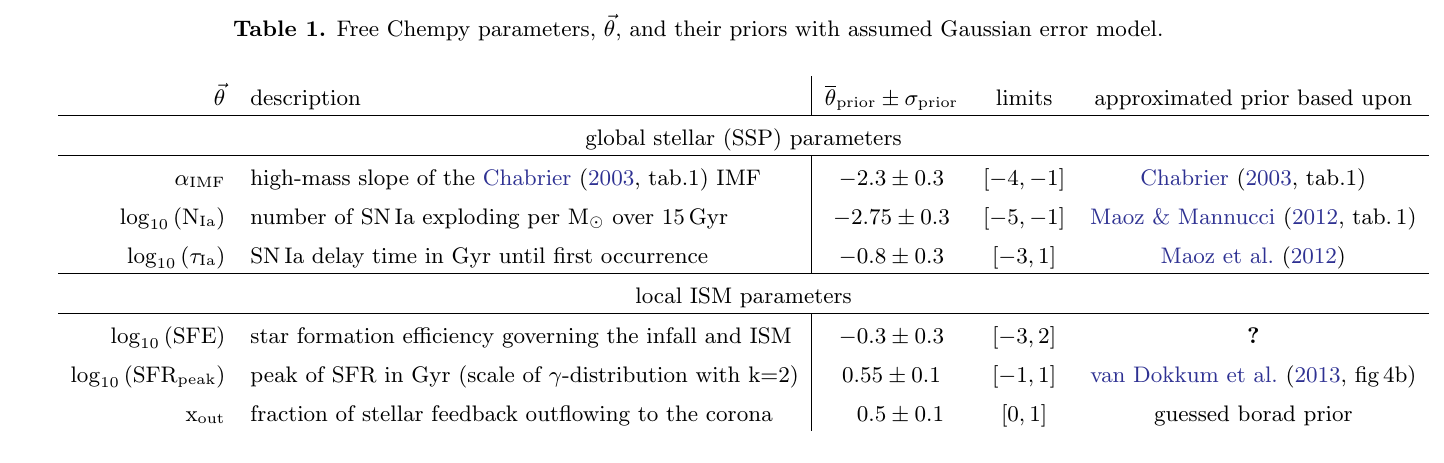
\includegraphics[width=\textwidth]{Prior.png}

 \tiny (Philcox \& Rybizki, in prep.)
\end{frame}

\subsection{Chempy Calculation}
\begin{frame}
\frametitle{\textit{Chempy}}
\framesubtitle{Calculation Schematic}
MCMC Parameter Optimization:
\hspace{50pt}
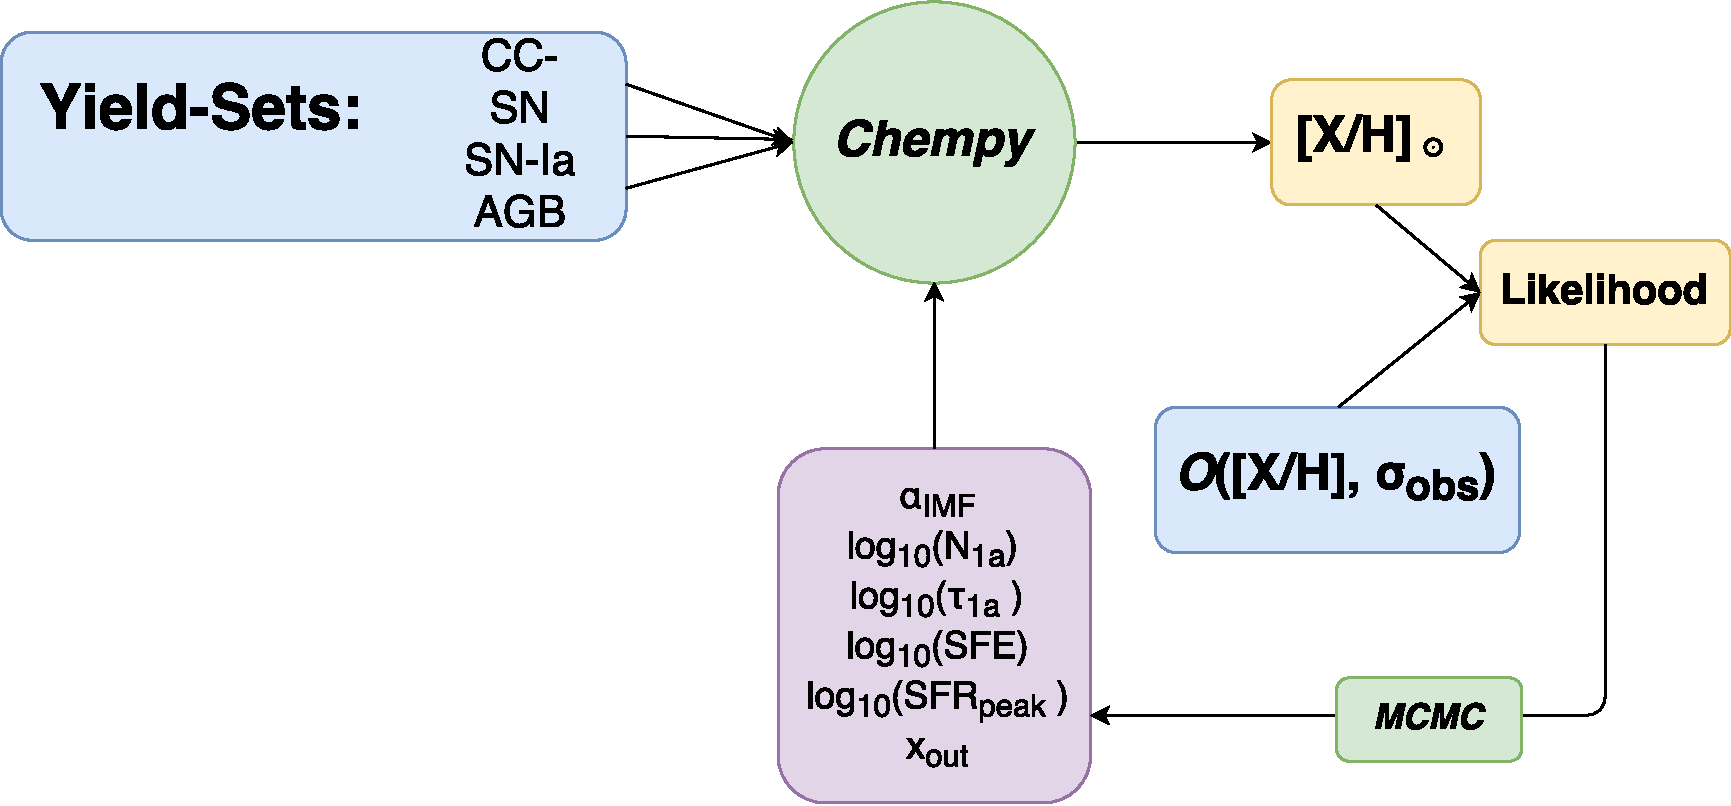
\includegraphics[width=\textwidth]{Chempy.pdf}
\end{frame}

\subsection{Error function}
\begin{frame}
\frametitle{\textit{Chempy}}
\framesubtitle{Error Function}
\begin{itemize}
\item For each element, we marginalize over the model error, $\sigma_\mathrm{model}$, to account for unmodelled effects.
\item Error function is a $\beta(x; k,1)$ function, for abundance $x$.
\item $k$-parameter controls the error strength (default = 3).
\end{itemize}
\begin{figure}
\centering
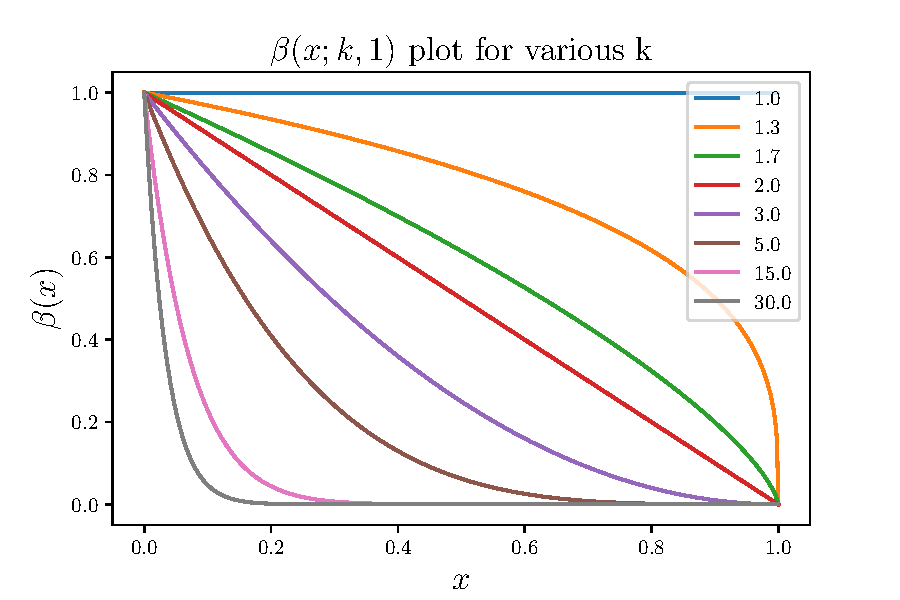
\includegraphics[width=0.7\textwidth]{beta.pdf}
\end{figure}
\end{frame}

\subsection{Posteriors}
\begin{frame}
\frametitle{\textit{Chempy} Posteriors}
\framesubtitle{Optimal parameter set}
Posteriors were calculated for two choices of yield sets (hyperparameters):
\begin{itemize}
\item  \textbf{CC-SN}: Nomoto et al. (2013)
\item \textbf{ SN-Ia}:  Seitenzahl et al. (2013) 
\item \textbf{AGB}: Karakas (2010) or Karakas (2016)
\vfill
\end{itemize}
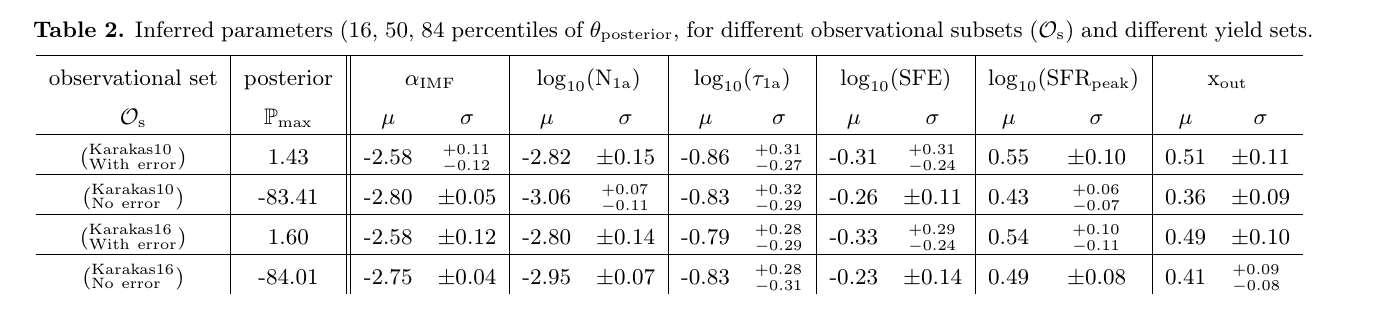
\includegraphics[width=\textwidth]{ChempyPosterior.png}

\tiny (Philcox \& Rybizki, in prep.)
\end{frame}

\begin{frame}
Output for Karakas (2016) AGB yields
\frametitle{\textit{Chempy}}
\framesubtitle{Corner Plot}
\begin{figure}
\centering
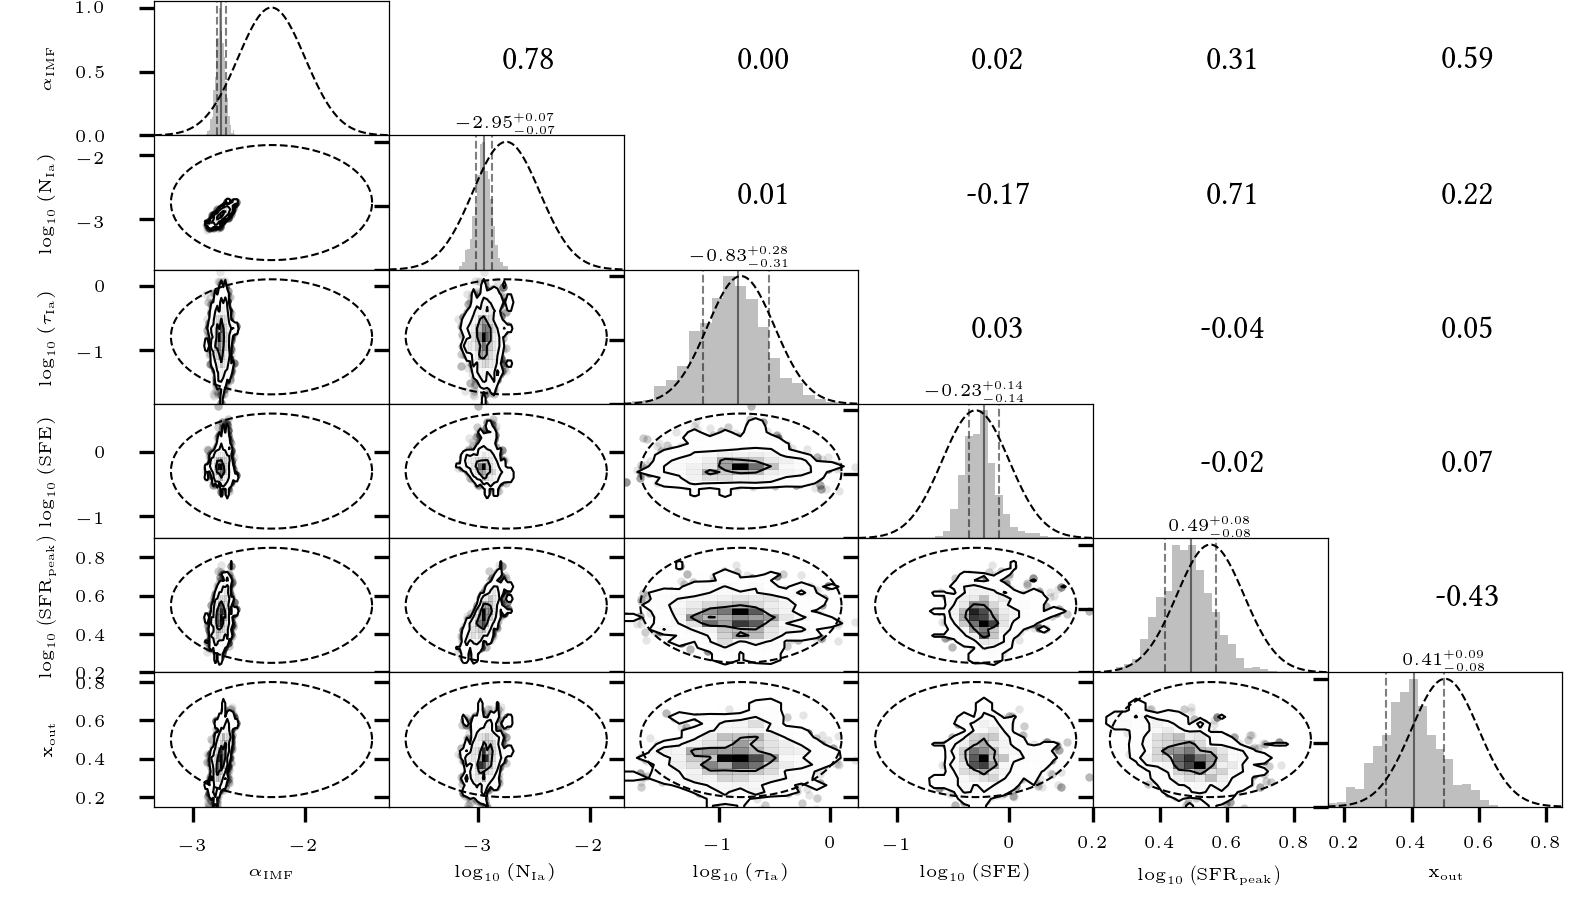
\includegraphics[width=\textwidth]{Karakas16ZeroError.png}
\end{figure}
\end{frame}

\begin{frame}
Output for Karakas (2016) AGB yields with $\beta$ error model
\frametitle{\textit{Chempy}}
\framesubtitle{Corner Plot  + Errors}
\begin{figure}
\centering
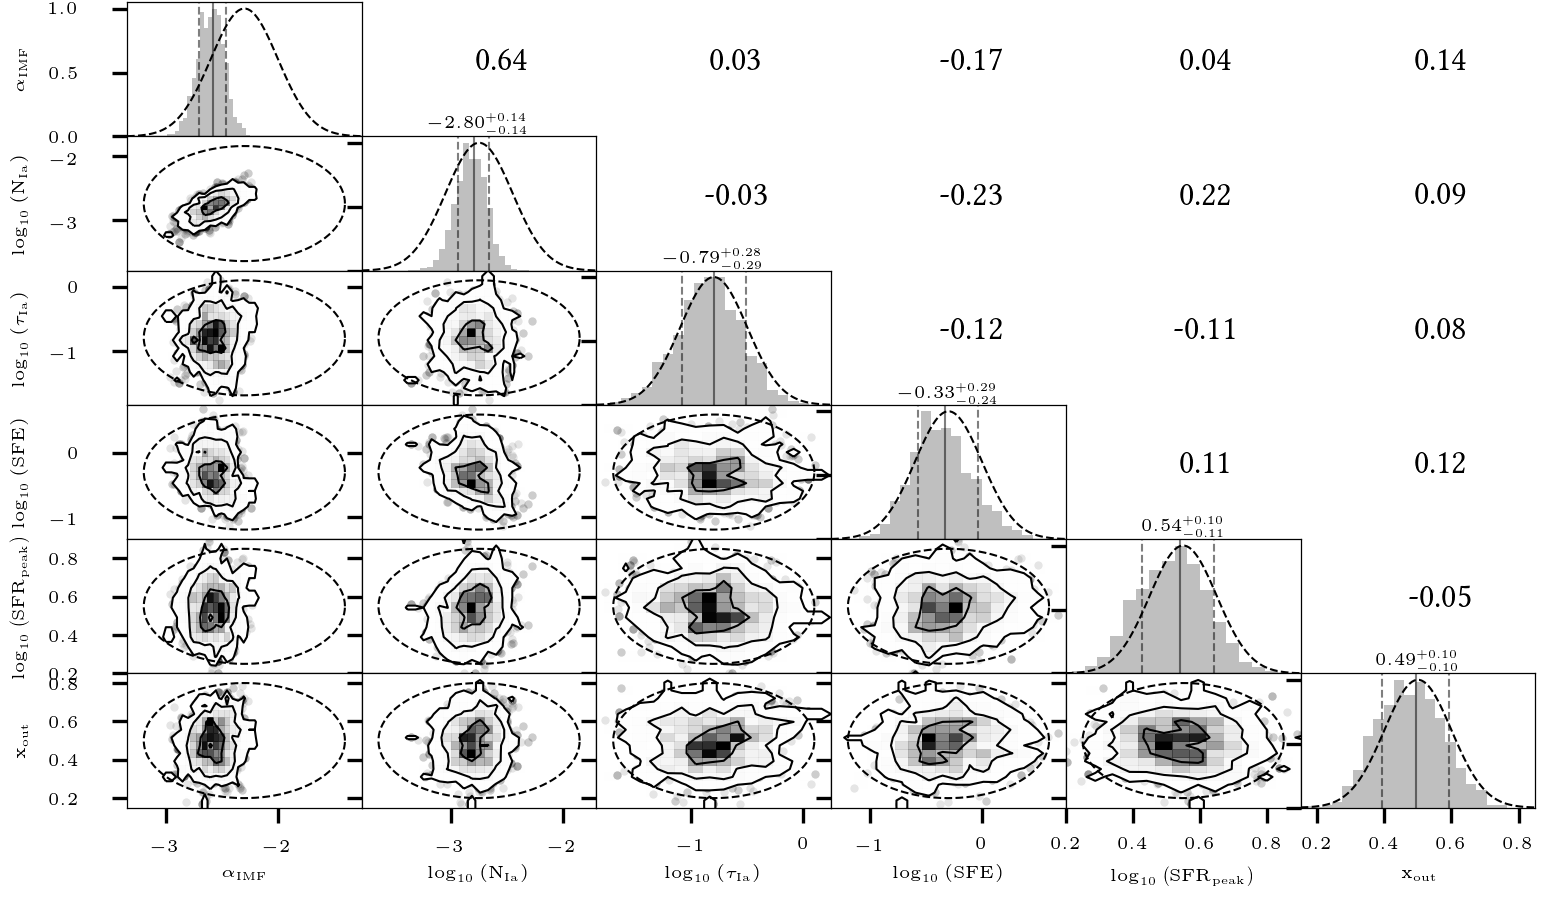
\includegraphics[width=\textwidth]{Karakas16.png}
\end{figure}
\end{frame}

\section{Neural Networks}
\subsection{Motivation}
\begin{frame}
\frametitle{Neural Networks}
\framesubtitle{Motivation}
\begin{itemize}
\item The\textit{ Chempy} code takes $\approx$ 3s to run per set of parameters queried
\item This is too slow for efficient MCMC sampling and future parameter-space integration:
\begin{itemize}
\item Train a neural network to predict the output abundances from input parameters
\item This runs in 7 ms here
\end{itemize}
\end{itemize}
\begin{figure}
\centering
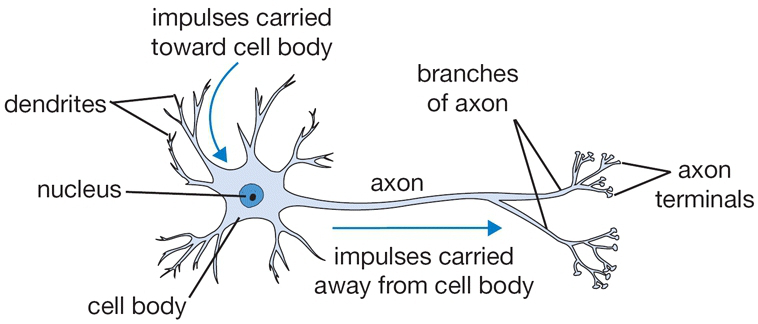
\includegraphics[width=0.6\textwidth]{neuron.png}
\end{figure}
\tiny Karparthy et al. (2017)
\end{frame}

\subsection{Network Structure}
\begin{frame}
\frametitle{Neural Networks}
\framesubtitle{Network Structure}
Network schematic: 
\begin{figure}
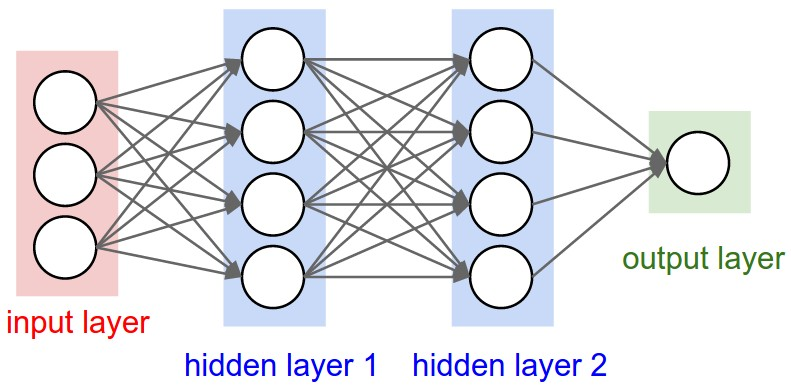
\includegraphics[width=0.6\textwidth]{neural_net2.png}
\end{figure}
\begin{tiny}
Karparthy et al. (2017)\\
\end{tiny}
Our implementation:
\begin{itemize}
\item 6 inputs (parameter vector $\theta$)
\item 22 outputs ([X/Fe] abundances)
\item 1 hidden layer with 30 neurons
\end{itemize}
\end{frame}

\subsection{Network Structure}
\begin{frame}
\frametitle{Neural Networks}
\framesubtitle{Network Structure}
\begin{itemize}
\item Network created using \textit{PyTorch} (\url{pytorch.org})
\item Settings used:
\begin{itemize}
\item Adam sampler (Kingma \& Ba 2014)
\item L1 loss function
\item $\tanh$ activator function
\item \textit{PyTorch}'s  \texttt{ReduceLROnPlateau} function
\item 5000 training epochs
\end{itemize}
\end{itemize}
\begin{figure}
\centering

\includegraphics[width = 0.5\textwidth]{index.png}
\end{figure}
\end{frame}

\subsection{Creating the Network}
\begin{frame}
\frametitle{Neural Networks}
\framesubtitle{Training the Network}
\begin{enumerate}
\item Create network architecture
\item Load $5^6$ element training data-set, with parameters evenly distributed in Gaussian prior space
\item Train neural network with data-set
\item Optimize learning rate using random 10,000 element verification data-set (0.003 here)
\item Test settings with a further random 10,000 element data-set
\end{enumerate}
\begin{figure}
\centering
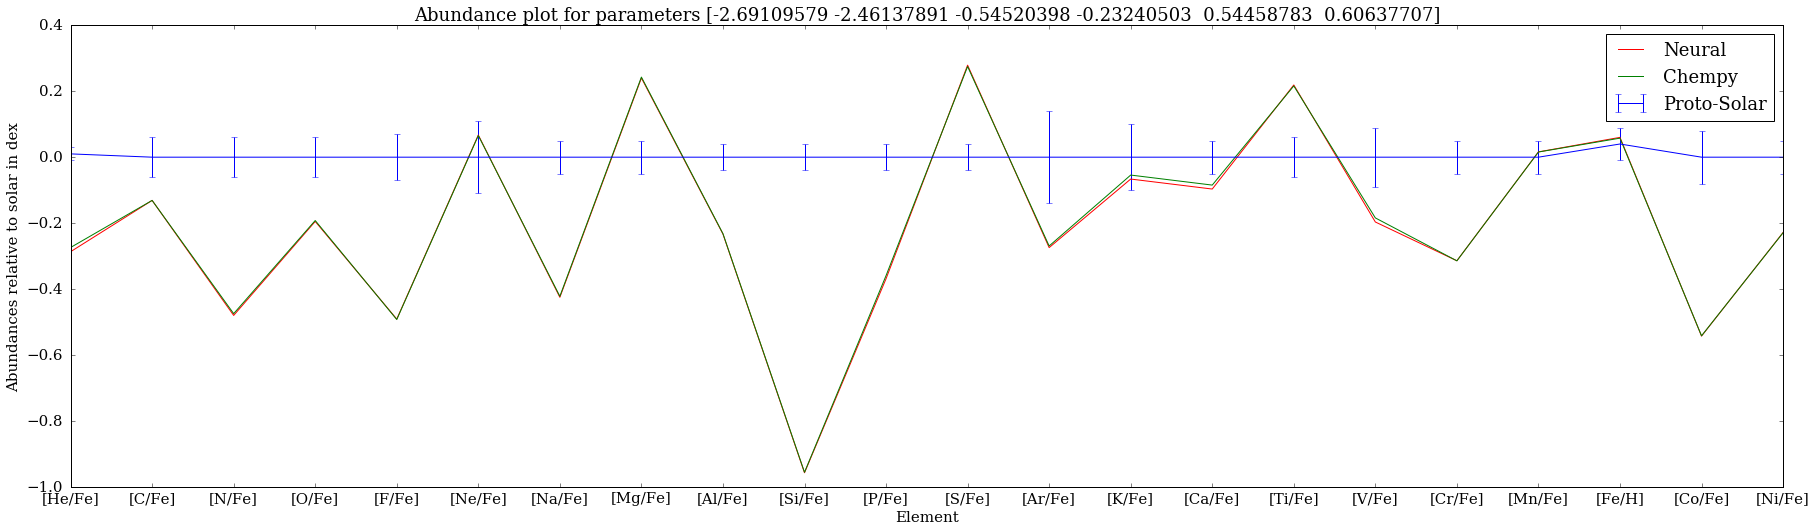
\includegraphics[width=\textwidth]{neural_abundances.png}
\end{figure}
\end{frame}

\subsection{Testing the Network}
\begin{frame}
\frametitle{Testing the Network}
\framesubtitle{Error Histogram}
\begin{figure}
\centering
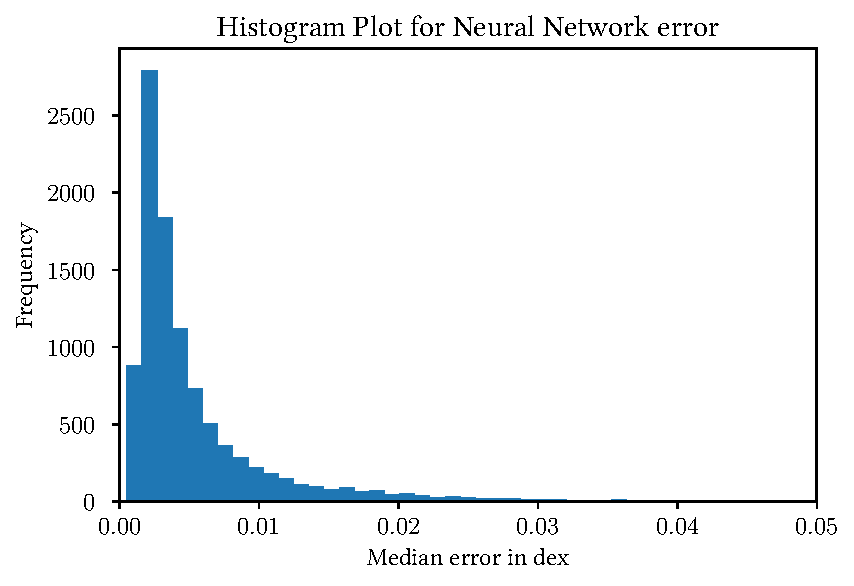
\includegraphics[width=0.8\textwidth]{neural_hist.pdf}
\end{figure}
\end{frame}

\begin{frame}
\frametitle{Testing the Network}
\framesubtitle{Median Element Error Corner Plot}
\begin{figure}
\centering
\includegraphics[width=\textwidth]{test_corner_parameter_plot.png}
\end{figure}
\end{frame}

\section{Creating an Objective Score}
\begin{frame}
\frametitle{How can we create an objective scoring for yield tables?}
\begin{itemize}
\item Use Bayes' factor to compare yield sets
\begin{eqnarray*}
K &=& \frac{K_1}{K_2};\\
K_k = \mathrm{P}(\mathcal{O}|\chi_k) &=& \int_{\vec{\theta}}\mathrm{P}(\mathcal{O}|\vec{\theta},\chi_k)p(\vec{\theta}) \mathrm{d}\vec{\theta}
\end{eqnarray*}
for observations $\mathcal{O}$ and yield sets $\chi$, with prior $p(\vec{\theta})$ on the parameters.
\item This is just the integrated posterior in 6 dimensions.
\item If $K \gg 1$ then $\chi_1$ better represents solar abundances than $\chi_2$.
\item Using the neural networks, we can calculate this integral using Monte Carlo methods e.g. \texttt{mcint} (Snowsill, 2011)
\end{itemize}
\end{frame}

\subsection{Objective Scoring Outline}
\begin{frame}
\frametitle{Objective Scoring Outline}
\framesubtitle{With \textit{Chempy}}
\begin{figure}
\centering
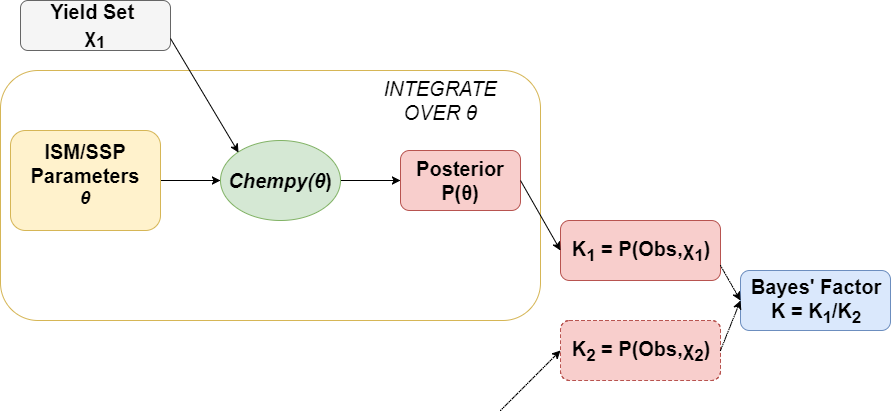
\includegraphics[width=\textwidth]{Neural.png}
\end{figure}
\end{frame}

\begin{frame}
\frametitle{Objective Scoring Outline}
\framesubtitle{With Neural Network}
\begin{figure}
\centering
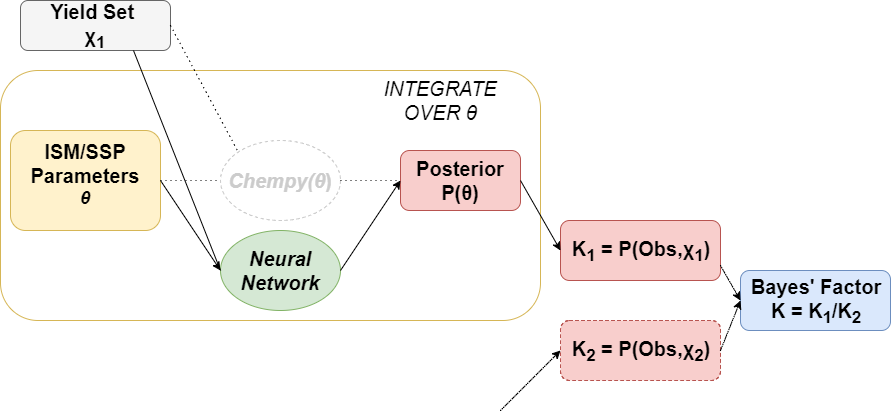
\includegraphics[width=\textwidth]{Neural2.png}
\end{figure}
\end{frame}

\subsection{Dealing with Errors}
\begin{frame}
\frametitle{Objective Scoring}
\framesubtitle{Elements \& Errors}
\begin{itemize}
\item Which elements should we fit for?
\begin{itemize}
\item Probably all elements else we introduce additional bias.
\end{itemize}
\item The model error in each element of \textit{Chempy} is not known. 
\item Currently we marginalize over the error during each posterior calculation, using a  $\beta$ model.
\begin{figure}
\centering
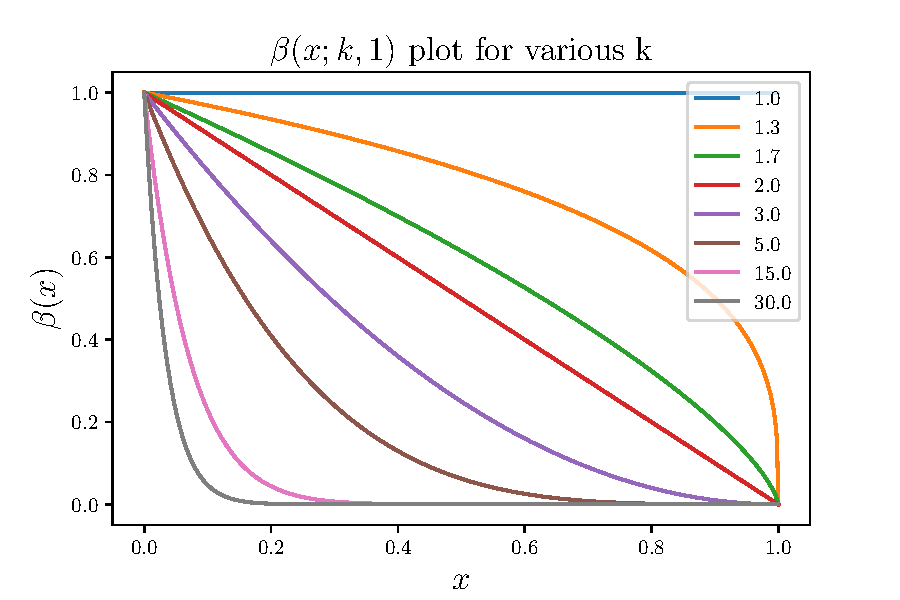
\includegraphics[width=0.8\textwidth]{beta.pdf}
\end{figure}
\end{itemize}
\end{frame}

\begin{frame}
\frametitle{Objective Scoring}
\framesubtitle{Elements \& Errors}
\begin{itemize}
\item One option:
\begin{itemize}
\item Parameterize the error using the $\beta(x,k,1)$ $k$-parameter
\item Calculate $K(k)$ across $k$-space
\item As $k\rightarrow \infty$, the error tends to 0
\item As $k\rightarrow 1$ the error tends to 1 dex
\end{itemize}
\item Any other suggestions?
\end{itemize}
\begin{figure}
\centering
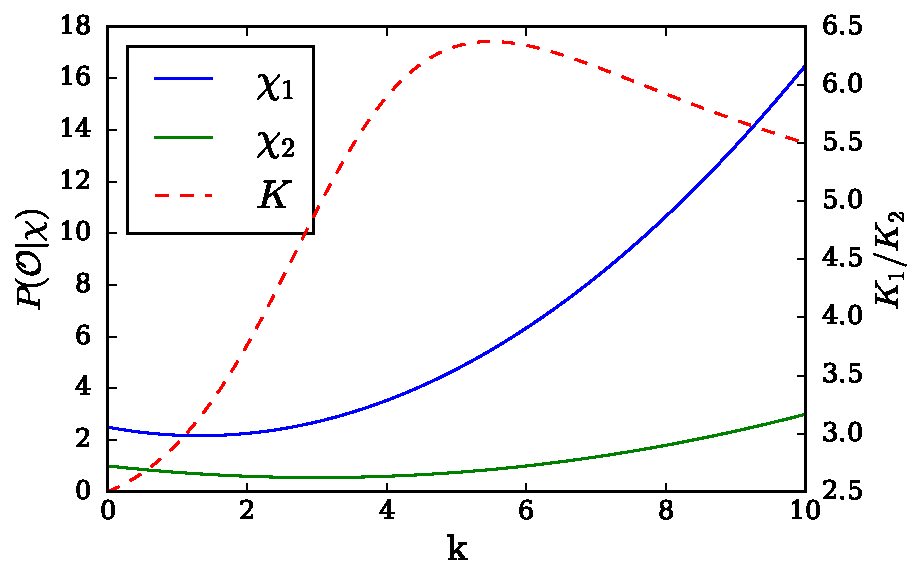
\includegraphics[width=0.6\textwidth]{Kplot.pdf}
\end{figure}
\end{frame}

\subsection{Further Work}
\begin{frame}
\frametitle{Further Work}
\begin{itemize}
\item Implement objective scoring function into \textit{Chempy}
\begin{itemize}
\item Widen the training data-set to span 3$\sigma$ per parameter
\item Retest neural network
\item Integrate over parameter space using Monte Carlo methods
\item Calculate objective score
\end{itemize}
\item Test approach on different sets of yield tables
\end{itemize}
\end{frame}

\end{document}
